\documentclass[12pt,aspectratio=169]{beamer}
\usepackage{tikz}
\usetheme{Madrid}
\setbeamertemplate{navigation symbols}{}
\title{Iterative refinement: experiments and bounds}
\subtitle{Generated interaction study}
\author{Research group}
\date{}
\year=2026\month=11\day=5
\newcommand{\fuzzlayerA}[1]{\textbf{#1}}
\newcommand{\fuzzterm}[1]{\fuzzlayerA{#1}}
\newcommand{\fuzzpair}[2]{\fuzzterm{#1}: #2}
\newcommand{\fuzzunit}{steps}
\let\fuzzoriginalunit\fuzzunit
\newcommand{\fuzzcoefficient}{4}
\newcommand{\fuzzscale}[2][\fuzzcoefficient]{#1\,#2}
\definecolor{fuzzpaint}{RGB}{255,0,255}
\definecolor{fuzzsecond}{RGB}{18,137,67}
\tikzset{fuzzvertex/.style={draw,rounded corners=1pt,fill=blue!10,inner sep=1pt,minimum width=.35cm,minimum height=.25cm}}
\begin{document}
\section{Iterative refinement}
\begin{frame}[t,shrink=5]{Iterative refinement}{Composed dependencies}
\fuzzpair{Experiment}{Timing: 12\fuzzunit; estimate $\fuzzscale{x}+\fuzzscale[2]{y}$.}\par
{\renewcommand{\fuzzunit}{samples}\let\fuzzterm\textit\fuzzpair{LocalScope}{Timing: 7\fuzzunit.}\par}
\fuzzpair{RestoredScope}{Timing: 11\fuzzunit.}\par
{\small\color{blue}\raggedright
\begin{enumerate}
\item \textrm{The next pass} must preserve the boundary conditions while revisiting dependent values. The next pass must preserve the boundary conditions while revisiting dependent values. The estimate is $\sum_{i=1}^{n}x_i$.
\item \textbf{A narrow column} can change line breaking even when the underlying expression is unchanged. The final diagram records the order in which information crosses the partition. The estimate is $x_i+x_{i+1}$.
\item \begin{alertblock}{Message passing}
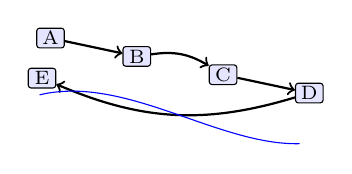
\begin{tikzpicture}[font=\scriptsize]
\begin{scope}[scale=0.8,rotate=-12]


\node[fuzzvertex] (g6n0) at (0.000,0) {A};
\node[fuzzvertex] (g6n1) at (1.400,0) {B};
\node[fuzzvertex] (g6n2) at (2.800,0) {C};
\node[fuzzvertex] (g6n3) at (4.200,0) {D};
\node[fuzzvertex] (g6n4) at (0.000,-0.65) {E};
\begin{scope}[xshift=.5pt,yshift=-.5pt]
\draw<2->[->,thick] (g6n0) -- (g6n1);
\draw<2->[->,thick] (g6n1) to[bend left=20] (g6n2);
\draw<2->[->,thick] (g6n2) -- (g6n3);
\draw<2->[->,thick] (g6n3) to[bend left=20] (g6n4);
\draw[blue] (0,-.9) .. controls (1.260,-.3) and (2.940,-1.1) .. (4.200,-.8);
\end{scope}
\end{scope}
\end{tikzpicture}
\end{alertblock}
\end{enumerate}
\par
{\footnotesize\color{teal}\raggedright
\begin{enumerate}
\item \textit{A local update} can change the measurements used by several neighboring components. The final diagram records the order in which information crosses the partition. The estimate is $\frac{a+b}{1+c}$.
\item \textit{The final diagram} records the order in which information crosses the partition.  The estimate is $x_i+x_{i+1}$.
\item 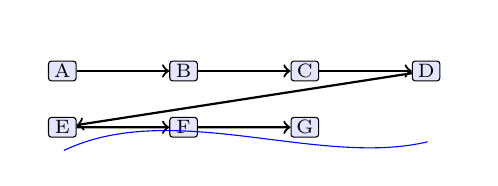
\begin{tikzpicture}[font=\scriptsize]
\begin{scope}[scale=1.1,rotate=0]
\clip (-.4,-1) rectangle (4.700,.5);

\node[fuzzvertex] (g11n0) at (0.000,0) {A};
\node[fuzzvertex] (g11n1) at (1.400,0) {B};
\node[fuzzvertex] (g11n2) at (2.800,0) {C};
\node[fuzzvertex] (g11n3) at (4.200,0) {D};
\node[fuzzvertex] (g11n4) at (0.000,-0.65) {E};
\node[fuzzvertex] (g11n5) at (1.400,-0.65) {F};
\node[fuzzvertex] (g11n6) at (2.800,-0.65) {G};
\begin{scope}[xshift=.5pt,yshift=-.5pt]
\draw<2->[->,thick] (g11n0) -- (g11n1);
\draw<2->[->,thick] (g11n1) -- (g11n2);
\draw<2->[->,thick] (g11n2) -- (g11n3);
\draw<2->[->,thick] (g11n3) -- (g11n4);
\draw<2->[->,thick] (g11n4) -- (g11n5);
\draw<2->[->,thick] (g11n5) -- (g11n6);
\draw[blue] (0,-.9) .. controls (1.260,-.3) and (2.940,-1.1) .. (4.200,-.8);
\end{scope}
\end{scope}
\end{tikzpicture}
\end{enumerate}\par}
\par
\begin{alertblock}{Constraint propagation}
\uncover<2->{\textrm{The next pass} must preserve the boundary conditions while revisiting dependent values. A local update can change the measurements used by several neighboring components. The estimate is $\alpha+\beta$.}
\end{alertblock}\par}
\par 
\begin{tikzpicture}[font=\scriptsize]
\fill<2-3>[fuzzpaint] (0,0) rectangle (.8,.3);
\fill<3->[fuzzsecond] (1,0) rectangle (1.8,.3);
\node[anchor=west] at (2,0.15) {Witness};
\end{tikzpicture}
\only<4>{}
\end{frame}\end{document}
